\documentclass[dvipdfmx,fleqn]{beamer}
\usepackage{amsmath,amsthm,amssymb}
\usepackage{algorithm,algpseudocode}
\graphicspath{{./figure/}{./plot/}}
\makeatletter
\def\input@path{{./figure/}{./table/}}
\makeatother
\usepackage[
sorting=debug,
style=ieee,backend=bibtex,
texencoding=utf8,bibencoding=utf8,
dashed=false,
isbn=false,url=false,doi=false,
sorting=debug
]{biblatex}
\addbibresource{References.bib}
\AtBeginBibliography{}
\setbeamertemplate{bibliography item}[text]
\usetheme{IMELAB}
\usefonttheme[onlymath]{serif}

\usepackage{bxdpx-beamer}
\usepackage{pxjahyper}
\usepackage{verbatim}
%\usepackage[absolute,overlay]{textpos}

\renewcommand{\kanjifamilydefault}{\gtdefault}
\renewcommand{\familydefault}{\sfdefault}

% Theorem
\uselanguage{japanese}
\languagepath{japanese}
\deftranslation[to=japanese]{Theorem}{定理}
\deftranslation[to=japanese]{Lemma}{補題}
\deftranslation[to=japanese]{Example}{例}
\deftranslation[to=japanese]{Examples}{例}
\deftranslation[to=japanese]{Definition}{定義}
\deftranslation[to=japanese]{Definitions}{定義}
\deftranslation[to=japanese]{Problem}{問題}
\deftranslation[to=japanese]{Solution}{解}
\deftranslation[to=japanese]{Fact}{事実}
\deftranslation[to=japanese]{Proof}{証明}
\def\proofname{証明}

% Caption
\renewcommand{\figurename}{図}
\renewcommand{\tablename}{表}

% Beamer Misc.
\usepackage{appendixnumberbeamer}
\setbeamertemplate{navigation symbols}{}
\setbeamertemplate{frametitle continuation}[from second][(続き)]
%\setbeamertemplate{note page}[plain] % 基本これで
\setbeamertemplate{note page}{ % ちょこっとカスタマイズ
  \vspace{.5em}
  \insertslideintonotes{.30}
  \hfill
  {\tiny ページ\insertframenumber{}/\inserttotalframenumber}
  \noindent\rule{\textwidth}{.5pt}
  {\scriptsize\insertnote}
}
\setbeameroption{show notes} % スライド+ノート
%\setbeameroption{hide notes} % スライドのみ
%\setbeameroption{show only notes} % ノートのみ

\title[媒介中心性更新法]{辺操作時の最短経路の更新を利用する \\ 媒介中心性更新法}
\author[里谷]{里谷 佳紀}
\institute[情数工研]{情報数理工学研究室}
\date[研究発表会]{2019年度修士論文研究発表会 \\ 2020年2月12日}

\begin{document}

%\makeIMELABtitle
{
  \setbeamertemplate{footline}[imelab]
  \begin{frame}
    \titlepage
    \note[item]{ノートなのだ}
    \note[item]{情報数理工学研究室の里谷が}
    \note[item]{辺操作時の最短経路の更新を利用する媒介中心性更新法}
    \note[item]{という題目で発表します}
    \note[item]{よろしくおねがいします}
  \end{frame}
}

\begin{frame}{概要}
  \begin{itemize}
  \item 背景
    \begin{itemize}
    \item ネットワークの中の重要なノードを見つけたい(アキレス腱)
    \item[] $\rightarrow$\alert{媒介中心性}はノードの重要さを表す
    \item Brandes法:媒介中心性の値を高速に計算する
    \item 現実のネットワークは\alert{絶えず変化し続ける}
    \item[] $\rightarrow$変化の影響を受ける部分だけを更新してさらに高速化
    \end{itemize}
  \item 提案手法
    \begin{itemize}
    \item 辺削除時に最短経路と共に媒介中心性を更新する手法
    \end{itemize}
    \begin{enumerate}
    \item 影響を受ける頂点の集合を計算
    \item 媒介中心性の値を影響を受ける分だけ\alert{減算}
    \item \alert{最短経路を更新}
    \item 媒介中心性の値を影響を受ける分だけ\alert{加算}
    \end{enumerate}
  \item 結果
    \begin{itemize}
    \item 計算量を比較$\rightarrow$Brandes法以下の計算量
    \item 実験により比較$\rightarrow$Brandes法の$14.67\%$の実行時間で更新可能
    \end{itemize}
  \end{itemize}
  \note[item]{まず発表の\alert{概要}を示します.}
  \note[item]{
    ネットワークの中の\alert{重要なノード}を見つけることはネットワーク解析において重要な課題です.
    重要なノードはアキレス腱のようなもので,しばしば不可欠な役割を果たします.
  }
  \note[item]{
    ノードの重要さを測る指標として\alert{媒介中心性}がよく用いられます.
  }
  \note[item]{
    媒介中心性の値を高速に計算する方法として\alert{Brandesのアルゴリズム}が知られてます.
  }
  \note[item]{
    しかし現実のネットワークはノードやリンクの挿入や削除によって絶えず\alert{その形を変化させ続け}ています.
    そのようなネットワークの媒介中心性を求める場合,変化の影響を受ける部分だけを更新してさらなる高速化が期待できます.
  }
  \note[item]{
    そこで,この研究では,最短経路の更新を利用して媒介中心性を更新する方法を提案し,評価します.
  }
  \note[item]{
    アルゴリズムは,まず,影響を受ける分だけ媒介中心性の値を減算したあと,最短経路を更新し,
    最後に影響を受ける分だけ媒介中心性の値を加算することで媒介中心性を更新します.
  }
  \note[item]{
    アルゴリズムの評価の結果,提案手法は,Brandes法以下の計算量を達成し,
    実ネットワークに対してBrandes法の$14.67\%$の実行時間で更新することを確認しました.
  }
\end{frame}

\section{背景・目的}
\begin{frame}[t]{研究背景 -- 媒介中心性}
  \begin{columns}
    \begin{column}{.59\textwidth}
      \begin{itemize}
      \item \alert{媒介中心性}\cite{05Freeman1977}:ノードの重要度を測る
      \item[] 例:鉄道網における駅
      \end{itemize}
      \medskip
      \begin{equation*}
        B_v=\sum_{s\neq v}\sum_{t\neq v,s}\frac{\sigma_{st}(v)}{\sigma_{st}}
      \end{equation*}
      \begin{itemize}\small
      \item $\sigma_{st}(v)$:$s$と$t$間の最短経路のうち\\$v$を通るものの数
      \item $\sigma_{st}$:$s$と$t$間の最短経路の数
      \end{itemize}
      \begin{itemize}
      \item 媒介中心性の値が高い\\$\rightarrow$\alert{多くの最短経路が通る}ので重要
      \item 単純法の計算量:\alert{$\mathcal{O}(|V|^3)$}
      \end{itemize}
    \end{column}
    \begin{column}{.4\textwidth}
      \centering
      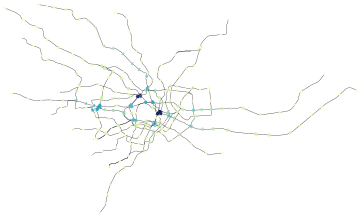
\includegraphics[angle=90,height=.77\textheight]{tokyo-metro-betweenness.png}
    \end{column}
  \end{columns}
  \hypercite{05Freeman1977}
  \note[item]{まず,\alert{研究背景}として媒介中心性について説明します.}
  \note[item]{
    媒介中心性とはネットワークのノードの\alert{重要度を測る}中心性と呼ばれる指標のひとつです.
  }
  \note[item]{
    媒介中心性の\alert{定義}はこちらの式で与えられます.
    ここで,$\sigma_{st}(v)$は$s$と$t$間の最短経路のうち$v$を通るものの数を,
    $\sigma_{st}$は$s$と$t$間の最短経路の数を表します.
  }
  \note[item]{
    あるノードの媒介中心性の値が高いと,そのノードの上に\alert{多くの最短経路}が通っているので,
    重要であると言えます.
  }
  \note[item]{
    例えば,こちらに路線図がありますが,媒介中心性の値が大きくなるほど色を濃くしています.
    ネットワークの中央付近のノードは最短経路が多く通っているため,濃く表示されています.
  }
  \note[item]{
    定義通りに媒介中心性を計算するときの計算量について考えると,
    この部分から,和は頂点数の二乗だけ繰り返されるので,計算量は頂点数の三乗のオーダです.
  }
\end{frame}

%\begin{frame}{媒介中心性の計算例}
%  \begin{columns}
%    \begin{column}{.6\textwidth}
%      頂点$v$の媒介中心性の値$B_v$は
%      \begin{flalign*}
%        B_v&=\sum_{s\neq v}\sum_{t\neq s,v}\frac{\sigma_{st}(v)}{\sigma_{st}}\\
%        &=\frac{\sigma_{wx}(v)}{\sigma_{wx}}+\frac{\sigma_{wy}(v)}{\sigma_{wy}}
%        +\frac{\sigma_{wz}(v)}{\sigma_{wz}}\\
%        &+\frac{\sigma_{xy}(v)}{\sigma_{xy}}+\frac{\sigma_{xz}(v)}{\sigma_{xz}}
%        +\frac{\sigma_{yz}(v)}{\sigma_{yz}}+\cdots\\
%        &=\frac{0}{1}+\frac{0}{1}+\frac{1}{1}+\frac{0}{1}+\frac{2}{2}+\frac{1}{1}\cdots\\
%        &=6.
%      \end{flalign*}
%      同様に,$B_w=B_y=2,\:B_x=B_z=0$.
%    \end{column}
%    \begin{column}{.39\textwidth}
%      \centering
%      \def\svgwidth{.9\linewidth}
%      \input{graph-bc.pdf_tex}
%    \end{column}
%  \end{columns}
%  \medskip
%  計算量:\alert{$\mathcal{O}(|V|^3)$}
%  \note[item]{ここで定義に従った媒介中心性の計算の例を示します.}
%  \note[item]{右に示したグラフの$v$の媒介中心性は,このように計算されます.}
%  \note[item]{
%    ここで,定義に従った方法で全ての頂点の媒介中心性の値を計算したときの計算量について考えます.
%  }
%  \note[item]{
%    総和記号の赤枠の部分から,和は頂点数$|V|$の二乗だけ繰り返されます.
%    そのため,全ての頂点の媒介中心性の値の計算の計算量は$|V|$の三乗オーダです.
%  }
%  \note[item]{
%    これでは,頂点数の増加とともに計算時間が膨大になり,巨大なネットワークの解析は困難です.
%  }
%\end{frame}

\begin{frame}{Brandesの定理}
  \begin{itemize}\small
  \item ペア依存度 $\delta_{st}(v)=\sigma_{st}(v)/\sigma_{st}$
  \item 依存度
    $\delta_{s\bullet}(v)=\sum_{t\neq s,v}\delta_{st}(v)$
  \item 媒介中心性
    $B_v=\sum_{s\neq v}\colorlet{oldcolor}{.}\usebeamercolor[fg]{alerted text}\fbox{$\color{oldcolor}\sum_{t\neq s,v}\sigma_{st}(v)/\sigma_{st}$}\color{oldcolor}=\sum_{s\neq v}\delta_{s\bullet}(v)$
  \item $\delta_{s\bullet}(v)$を高速に計算したい
  \end{itemize}
  \medskip
  \begin{theorem}[Brandes \footcite{06Brandes2001}]\rm
    \label{th:implicit-dependency}
    グラフ$G=(V,E)$の異なる頂点$s,v$について,頂点$v$の$s$に対する依存度$\delta_{s\bullet}(v)$は次式を満たす.
    \begin{equation*}
      \delta_{s\bullet}(v)=\sum_{(v,w)\in E_s}\frac{\sigma_{sv}}{\sigma_{sw}}(1+\delta_{s\bullet}(w)).
    \end{equation*}
    ただし,$E_s$は$s$から各頂点への最短経路の辺集合である.
  \end{theorem}
  \begin{flushright}
    \alert{次で例を説明}
  \end{flushright}
  \note[item]{
    媒介中心性の値を高速に計算するため,Brandesは\alert{依存度}と呼ばれる値を高速に計算する方法を提案しました.
  }
  \note[item]{
    \alert{依存度}とは,ペア依存度$\sigma_{st}(v)/\sigma_{st}$を$t$について総和を取ったものです.
    依存度の定義を使うと,媒介中心性の定義のこの部分が依存度に置き換わります.
  }
  \note[item]{
    依存度を\alert{高速に計算}するため,Brandesは次の定理を示しました.
    この定理は,$v$の依存度は最短経路上で$v$の一つ後の頂点$w$の依存度から計算
    出来ることを示しています.
  }
\end{frame}

\begin{frame}{Brandesのアルゴリズム}
  \begin{columns}
    \begin{column}{.49\textwidth}
      右図において
      \begin{equation*}\small
        \begin{aligned}
          \delta_{s\bullet}(v)&=\frac{\sigma_{sv}}{\sigma_{sw_1}}(1+\delta_{s\bullet}(w_1)) \\
          &+\frac{\sigma_{sv}}{\sigma_{sw_2}}(1+\delta_{s\bullet}(w_2)) \\
          &+\frac{\sigma_{sv}}{\sigma_{sw_3}}(1+\delta_{s\bullet}(w_3))
        \end{aligned}
      \end{equation*}
    \end{column}
    \begin{column}{.49\textwidth}
      \centering
      \def\svgwidth{.9\columnwidth}
      \input{implicit-dependency.pdf_tex}
    \end{column}
  \end{columns}
  \medskip
  \begin{enumerate}
  \item $s$からの最短経路$E_s$を計算
  \item 最短距離の降順に頂点を走査($w$とする)
  \item $(v,w)$が最短経路に含まれるような$v$に対して
  \item[] $\delta_{s\bullet}(v)\gets\delta_{s\bullet}(v)+\colorlet{oldcolor}{.}\usebeamercolor[fg]{alerted text}\fbox{$\color{oldcolor}\sigma_{sv}/\sigma_{sw}(1+\delta_{s\bullet}(w))$}\color{oldcolor}$
  \end{enumerate}
  計算量:\alert{$\mathcal{O}(|V|^2\log |V|+|V||E|)$}
  \note[item]{
    Brandesの定理を使った依存度の\alert{計算の例}を示します.
    $v$の依存度は,定理からこの式で計算できます.
    ここで,最短経路の上で$v$のひとつ後ろは$w_1,w_2,w_3$です.
  }
  \note[item]{
    Brandesのアルゴリズムの\alert{手順}を簡単に説明します.
    まず$s$からの最短経路を計算します.
    その後,$s$から遠い順に頂点$w$を走査し,$w$の一つ前の$v$に対して,
    この式で$v$の依存度を更新します.
  }
  \note[item]{
    Brandes法で媒介中心性を計算するときの\alert{計算量}はこれで,
    疎なネットワークに対してある程度高速に媒介中心性を計算できます.
  }
\end{frame}

\begin{frame}{時変ネットワークの媒介中心性}
  \begin{columns}
    \begin{column}{.5\textwidth}
      \begin{itemize}
      \item Brandes法は変化しないネットワークに対する方法
      \item 現実のネットワークは変化する
      \item[] \alert{時変ネットワーク}\cite{18Holme2012}
      \item[] 例:道路の建設
      \item 時変ネットワークの媒介中心性
      \item[] 変化する頂点は少ない
      \item[] 変化分を効率的に計算したい
      \end{itemize}
    \end{column}
    \begin{column}{.5\textwidth}
      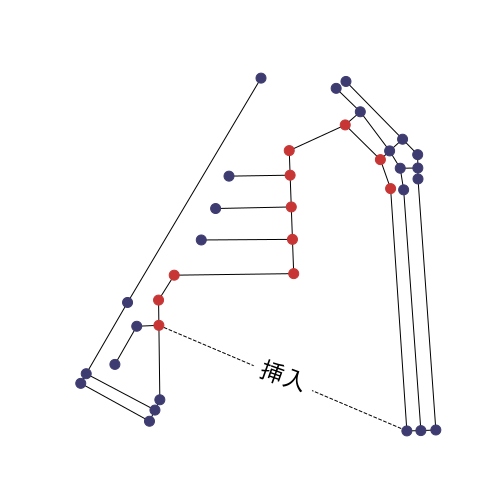
\includegraphics[width=.9\columnwidth]{road-sta.pdf}
    \end{column}
  \end{columns}
  \hypercite{18Holme2012}
  \note[item]{
    先ほど説明したBrandesのアルゴリズムは,ネットワークにノードやリンクが追加されない,
    ネットワークに対して媒介中心性の値を計算します.
  }
  \note[item]{
    しかし現実のネットワークは,例えば道路の建設などによって,
    その形が絶えず変化する\alert{時変ネットワーク}です.
  }
  \note[item]{
    このようなネットワークに対しては,媒介中心性が\alert{変化する分だけ}を計算することで,
    より高速に動作すると期待できます.
  }
  \note[item]{
    \alert{例えば},このネットワークにこのリンクを追加した場合,追加によって媒介中心性の値が
    変化するノードは赤く示したこれらのノードで,ネットワーク全体のノードに比べて
    三割程度です.
  }
\end{frame}

\begin{frame}{研究目的}
  \begin{itemize}
  \item 辺削除時の媒介中心性更新法
    \begin{itemize}
    \item 最短経路と共に媒介中心性を更新(\alert{最短経路更新法}がベース)
    \item 他の手法(専用データ構造を用いた手法,近似法)
    \end{itemize}
  \end{itemize}
  \begin{center}
    \small
    \begin{tabular}{lll}
      \hline
      最短経路更新法 & 最悪時間計算量 & \alert{最悪空間計算量} \\ \hline
      RamalingamとReps\cite{24Ramalingam1996} & $\mathcal{O}(|V|^2\log|V|+|E||V|)$ & $\mathcal{O}(|V|^2)$ \\ \hline
      DemetrescuとItaliano\cite{28Demetrescu2003} & $\mathcal{O}(|V|^2\log^2|V|)$ & $\mathcal{O}(|V|^3)$ \\ \hline
    \end{tabular}
  \end{center}
  \begin{itemize}
  \item Demetrescu-Italiano法に基づく媒介中心性更新法\footcite{29Nasre2014b}
  \item[] 最悪空間計算量:$\mathcal{O}(|V|^3)$
  \item Ramalingam-Reps法を用いることで\alert{空間計算量を削減}
  \end{itemize}
  \begin{block}{}
    RamalingamとRepsの最短経路更新法を利用する \\
    辺削除時の媒介中心性更新法の提案と評価
  \end{block}
  \note[item]{
    そのため時変ネットワークの媒介中心性を更新する方法が提案されてきました.
    その中でも,最短経路と共に更新する方法も提案されています.
    このような方法は,\alert{最短経路を更新する方法}に基づいています.
  }
  \note[item]{
    こちらに,\alert{最短経路を更新}する代表的な方法を示します.
  }
  \note[item]{
    \alert{Demetrescu-Italiano法}に基づく媒介中心性更新法がNasreらによって提案されましたが,
    最悪空間計算量は頂点数の三乗のオーダで,大規模なネットワークの解析には不向きです.
  }
  \note[item]{
    一方,Ramalingam-Reps法の最悪空間計算量は頂点数の二乗オーダで,
    この方法を基にすと\alert{空間計算量を抑えられる}と期待できます.
  }
  \note[item]{
    そこで,この研究は,RamalingamとRepsの最短経路更新アルゴリズムに基づく,
    辺削除時の媒介中心性更新法の提案と評価を目的とします.
  }
\end{frame}
  
\section{提案アルゴリズム}
\begin{frame}[allowframebreaks]{提案アルゴリズム}
  記号について
  \begin{itemize}\small
    \item \alert{$S(t)$}:辺削除によって$t$への最短経路が変化する頂点の集合
    \item \alert{$T(s)$}:辺削除によって$s$からの最短経路が変化する頂点の集合
    \item \alert{$\Delta_{s\bullet}(x)$}$=\sum_{t\in T(s)}\delta_{st}(x)$,
      \alert{$\Delta'_{s\bullet}(x)$}$=\sum_{t\in T(s)}\delta'_{st}(x)$:
    \item[] 削除の影響を受けるペア依存度の総和\footcite{31Bergamini2017}
    \item \alert{$\tau(s)$}$=T(s)\cup\{t|\Delta_{s\bullet}(t)>0\}$,
      \alert{$\tau'(s)$}$=T(s)\cup\{t|\Delta'_{s\bullet}(t)>0\}$:
    \item[] アルゴリズムによって走査された頂点の集合
  \end{itemize}
  \medskip
  アルゴリズムの大まかな流れ
  \begin{enumerate}
  \item 影響を受ける頂点($S(v)$と$T(u)$)を計算
  \item $B_x$を$\sum_{s\neq x}\Delta_{s\bullet}(x)$だけ減少
  \item 最短経路($d_{st}$と$\sigma_{st}$)を更新
  \item $B_x$を$\sum_{s\neq x}\Delta'_{s\bullet}(x)$だけ増加
  \end{enumerate}
  \begin{flushright}
    \alert{次は結果を示します}
  \end{flushright}

%  \begin{algorithmic}\footnotesize
%    \ForAll{$s\in S(v)$}
%    \Comment{\alert{影響を受ける頂点を計算}}
%    \State $\textproc{DecreaseBetweenness}(s)$
%    \Comment{\alert{$B_x$を$\sum_{s\neq x}\Delta_{s\bullet}(x)$だけ減少}}
%    \State $\textproc{UpdateSSSP}(s)$
%    \Comment{\alert{$d_{st}$と$\sigma_{st}$を更新}}
%    \State $\textproc{IncreaseBetweenness}(s)$
%    \Comment{$B_x$を$\sum_{s\neq x}\Delta'_{s\bullet}(x)$だけ増加}
%    \EndFor
%    \ForAll{$t\in T(u)$}
%    \Comment{影響を受ける頂点を計算}
%    \State $\textproc{UpdateSTSP}(t)$
%    \Comment{$d_{st}$と$\sigma_{st}$を更新}
%    \EndFor
%  \end{algorithmic}
  \note[item]{本研究で\alert{提案するアルゴリズム}について簡単に説明します.}
  \note[item]{
    $S(t)$と$T(s)$はそれぞれ辺削除によって$t$への,
    および$s$からの\alert{最短経路が変化する頂点の集合}とします.
  }
  \note[item]{
    さらに$\Delta_{s\bullet}(x)$と$\Delta_{s\bullet}(x)$をこの通り定義します.
    これは削除の\alert{影響を受けるペア依存度の総和}です.
  }
  \note[item]{
    アルゴリズムの大まかな流れは以下です.
    初めに$\Delta_{s\bullet}(x)$を求めて,媒介中心性の値$B_x$から減算します.
    次に,削除時の最短経路を更新します.
    最後に$\Delta'_{s\bullet}(x)$を求めて,媒介中心性の値$B_x$に加算します.
  }
\end{frame}

\section{性能評価}
\begin{frame}[allowframebreaks]{Brandes法との性能比較(人工ネットワーク)}
  \begin{columns}
    \begin{column}{.5\textwidth}
      \begin{itemize}
      \item 実験について
        \begin{itemize}
        \item 2種のネットワークモデル
        \item 平均次数$\langle k\rangle=4$
        \item ノード数$n\in\{100,\ldots,1000\}$
        \item $50$個のネットワーク
        \item $100$試行繰り返し
        \end{itemize}
        \medskip
      \item 提案手法の方が高速に動作する
      \item 実行時間の増加がBrandes法より緩やか
      \item[] $\rightarrow$\alert{走査する頂点の数の増加が緩やか}
      \end{itemize}
    \end{column}
    \begin{column}{.5\textwidth}
      \includegraphics[width=.9\columnwidth]{exp-artificial.pdf}
    \end{column}
  \end{columns}
  \note[item]{
    ここで,実験によって提案手法とBrandes法の性能を比較します.
    まず,\alert{人工ネットワークに対して性能比較}を行います.
    実験をこのような設定で行いました.
  }
  \note[item]{
    結果はこちらの図です.図より,どちらのネットワークモデルに対しても
    \alert{提案手法の方が高速に}動作することがわかります.
  }
  \note[item]{
    また,ノード数の増加に伴う実行時間の増加はBrandes法より緩やかであることもわかります.
    このことから,\alert{走査する頂点数の増加も抑えられている}ことが推測されます.
  }
\end{frame}

\begin{frame}[allowframebreaks]{Brandes法との性能比較(実ネットワーク)}
  \begin{columns}
    \begin{column}{.5\textwidth}
      \begin{itemize}
      \item 実験について
        \begin{itemize}
        \item SNAP\cite{32Leskovec2016}のデータセット
        \item $20$試行繰り返し
        \item 中央値を比較
        \end{itemize}
      \item ネットワークによって性能向上はまちまち
      \item 相対実行時間の
        \begin{itemize}
        \item 最小値:$5.78\%$
        \item 最大値:$29.05\%$
        \item 幾何平均:$14.67\%$
        \end{itemize}
      \end{itemize}
    \end{column}
    \begin{column}{.5\textwidth}
      \includegraphics[width=.9\columnwidth]{exp-real.pdf}
    \end{column}
  \end{columns}
  \hypercite{32Leskovec2016}
  \note[item]{
    次に,\alert{実ネットワーク}に対して性能比較を行います.
    実験をこのような設定で行いました.
    結果はこちらの図です.
  }
  \note[item]{
    図はそれぞれのネットワークに対して,Brandes法の実行時間を$1$としたときの
    提案手法の\alert{実行時間の相対値}を表しています.
  }
  \note[item]{
    図より,全てのネットワークに対して,提案手法の方が高速に動作していることがわかります.
    しかし,ネットワークによって\alert{提案手法の効果はまちまち}です.
    最も良い場合で$5.78\%$の時間で完了しますが,最も悪い場合で$29.05\%$の時間で完了します.
    幾何平均によると$14.67\%$の時間で実行できます.
  }
\end{frame}

\begin{frame}{時間計算量の評価}
  \begin{itemize}\small
    \item $|W|$:集合$W$の要素数,$||W||$:$W$の頂点と接続する辺の数
    \item 媒介中心性を増減させるアルゴリズムの時間計算量
    \begin{equation*}
      \mathcal{O}\left(\sum_{s\in S(v)}\left(\|\tau(s)\|+|\tau(s)|\log|\tau(s)|+\|\tau'(s)\|+|\tau'(s)|\log|\tau'(s)|\right)\right)
    \end{equation*}
  \item[] \alert{$S(v)=\tau(s)=\tau'(s)=V$}のときBrandesのアルゴリズムの計算量と同じ
    \item 最短経路を更新するアルゴリズムの時間計算量
    \begin{equation*}
      \mathcal{O}\left(\sum_{s\in S(v)}\|T(s)\|\log|T(s)|+\sum_{t\in T(u)}\|S(t)\|\log|S(t)|\right)
    \end{equation*}
  \item[] \alert{$S(v)=T(u)=V$}のときDijkstraのアルゴリズムの計算量と同じ
  \item 通常は$V$より小さい$\rightarrow$\alert{高速に動作}
  \end{itemize}
  \note[item]{ここでは,\alert{時間計算量}を既存のアルゴリズムのものと比較します.}
  \note[item]{
    \alert{媒介中心性を増減}させるアルゴリズムの時間計算量はこちらです.
    この計算量は,この条件を満たすとき,Brandesのアルゴリズムと同じ計算量になります.
  }
  \note[item]{
    \alert{最短経路を更新}するアルゴリズムの時間計算量はこちらです.
    この計算量も,この条件を満たすとき,Dijkstraのアルゴリズムと同じ計算量になります.
  }
  \note[item]{
    条件の頂点集合は頂点集合$V$の部分集合で,通常は$V$より小さくなるので,
    その分高速に動作します.
  }
\end{frame}

\section{アルゴリズムの詳細}
\begin{frame}[allowframebreaks]{提案アルゴリズム}
  記号について
  \begin{itemize}\small
    \item 辺$(u,v)$が削除されたと考える
    \item 記号$'$:削除後であることを表す(例:$G'$)
  \end{itemize}
  \medskip
  アルゴリズムの大まかな流れ
  \begin{enumerate}
  \item 影響を受ける頂点($S(v)$と$T(u)$)を計算
  \item $B_x$を$\sum_{s\neq x}\Delta_{s\bullet}(x)$だけ減少
  \item 最短経路($d_{st}$と$\sigma_{st}$)を更新
  \item $B_x$を$\sum_{s\neq x}\Delta'_{s\bullet}(x)$だけ増加
  \end{enumerate}
  \note[item]{以降,本研究で提案するアルゴリズムについて説明します.}
  \note[item]{グラフから辺$(u,v)$が削除されたと考えます.}
  \note[item]{
    削除後の諸量にプライム記号をつけて,それが削除後であることを明示します.
    例えば,削除後のグラフ$G$は$G'$で表します.
  }
  \note[item]{
    $S(t)$と$T(s)$はそれぞれ辺削除によって$t$への,および$s$からの最短経路が変化する頂点の集合とします.
    $S(t)$と$T(s)$の具体的な内容はあとで示します.
  }
  \note[item]{
    さらに$\Delta_{s\bullet}(x)$をこの通り定義します.
    これは削除の影響を受けるペア依存度$\delta_{st}(x)$の総和です.
  }
  \note[item]{
    アルゴリズムの大まかな流れは以下です.
    初めに影響を受ける頂点に対するペア依存度の総和を求めて,媒介中心性の値$B_x$から減算します.
    次に,削除時の最短経路を更新します.
    最後に影響を受ける頂点に対するペア依存度の総和を求めて,媒介中心性の値$B_x$に加算します.
  }
\end{frame}

\begin{frame}{影響を受ける頂点}
  $T(x)$と$S(x)$の具体的な内容を求める
  \begin{lemma}
    頂点$s,t$に対して,$E_{st}'\neq E_{st}$であるための必要十分条件は$d_{su}+l_{uv}+d_{vt}=d_{st}$を満たすことである.
  \end{lemma}
  \begin{columns}[T]
    \begin{column}{0.60\textwidth}
      \begin{itemize}
      \item $E_{st}'\neq E_{st}$ならば,$(u,v)$は最短経路の上にある
      \item すると,$d_{su}+l_{uv}+d_{vt}=d_{st}$が成り立つ
      \end{itemize}
    \end{column}
    \begin{column}{0.38\textwidth}
      \centering
      \def\svgwidth{.9\columnwidth}
      \input{condition-affection.pdf_tex}
    \end{column}
  \end{columns}
  \begin{itemize}
  \item $T(x)=\{t\,|\,d_{xt}=d_{xu}+l_{uv}+d_{vt}\}$
  \item $S(x)=\{s\,|\,d_{sx}=d_{su}+l_{uv}+d_{vx}\}$
  \end{itemize}
  両方とも,\alert{深さ優先探索}で計算可能
  \note[item]{ここで$S(x)$と$T(x)$の具体的な内容を求めます.}
  \note[item]{削除によって最短経路が変化する頂点ペアの条件について,こちらの補題を示しました.}
  \note[item]{
    頂点$s,t$に対して,最短経路が変化するための必要十分条件はこちらの式を満たすことです.
  }
  \note[item]{
    その根拠は,最短経路が変化するならば,削除される辺$(u,v)$は最短経路の上にあり,
    すると,この式が成り立つためです.
  }
  \note[item]{
    この補題によって,$S(x)$と$T(x)$の具体的な内容をこちらの通りに定義できます.
  }
  \note[item]{
    実際に内容を求めるには,削除される辺に接続する頂点$u$または$v$を始点として,
    深さ優先探索によって求められます.
  }
\end{frame}

\begin{frame}{媒介中心性の増減}
  増減のため各$s\in S(v)$の$\Delta_{s\bullet}(x)$を求める
  \begin{theorem}[Bergamini et al.\cite{31Bergamini2017}]\small
    任意の$s\in S(v)$と$x\in V$について,次式が成り立つ.
    \begin{equation*}
      \Delta_{s\bullet}(x)
      =\sum_{y\in\mathcal{S}_{G_s}(x)\cap T(s)}\frac{\sigma_{sx}}{\sigma_{sy}}(1+\Delta_{s\bullet}(y))
      +\sum_{y\in\mathcal{S}_{G_s}(x)\setminus T(s)}\frac{\sigma_{sx}}{\sigma_{sy}}\Delta_{s\bullet}(y)
    \end{equation*}
  \end{theorem}
  \begin{columns}[T]
    \begin{column}{.49\textwidth}
      \begin{itemize}
      \item Brandesのアルゴリズムと同様に$s$から遠い順に走査する
      \item $s$と$t\in T(s)$の最短経路の間にある頂点のみを走査する
      \item $y\in T(s)$か$y\notin T(s)$かで加算する値は異なる
      \end{itemize}
      $\Delta'_{s\bullet}(x)$も同様に計算可能
    \end{column}
    \begin{column}{.45\textwidth}
      \centering
      \def\svgwidth{.9\columnwidth}
      \input{calculate-affected-delta.pdf_tex}
    \end{column}
  \end{columns}
  \note[item]{
    次は影響を受ける頂点のペア依存度の総和である$\Delta_{s\bullet}(x)$を求める
    方法について説明します.
  }
  \note[item]{
    $\Delta_{s\bullet}(x)$について,この式が成り立つことが知られています.
    この式は,影響を受ける頂点の,$x$についてのペア依存度の総和は,
    最短経路上で$x$の後継の頂点についての$\Delta_{s\bullet}$から求められることを示しています.
  }
  \note[item]{
    この式を利用して$\Delta_{s\bullet}(x)$を求めるには,
    Brandesのアルゴリズムと同様に,$s$から遠い順に走査します.
  }
  \note[item]{
    ただし,Brandesのアルゴリズムでは全頂点を走査したのに対し,
    この方法では,影響を受ける頂点と,$s$とそれらの最短経路上にある頂点のみを走査します.
  }
  \note[item]{$\Delta'_{s\bullet}(x)$も同様に計算できます.}
\end{frame}

\begin{frame}{辺削除時の最短経路更新法}
  \begin{itemize}
  \item 更新後の距離の昇順に計算する必要がある
  \item[] しかしそのような並びは\alert{自明ではない}
  \item Ramalingam-Reps法\footcite{24Ramalingam1996}に基づき正しい順序で最短経路を更新する
  \end{itemize}
  \begin{columns}
    \begin{column}{.60\textwidth}
      \begin{enumerate}
      \item $x\in T(s)$のうち,$y\notin T(s)$を先行にもつ$x$はすぐに更新可能
      \item その距離と最短経路数はそれぞれ
        \begin{equation*}
          \begin{aligned}
            d'_{sx}&=\min\{d_{sx}+l_{xy}|y\in\mathcal{P}(x)\setminus T(s)\} \\
            \sigma'_{sx}&=\sum_{y\in \mathcal{P}_{G_s}(x)}\sigma_{sy}
          \end{aligned}
        \end{equation*}
      \item 以降,更新が完了した頂点から広げるように距離と最短経路数を更新
      \end{enumerate}
    \end{column}
    \begin{column}{.39\textwidth}
      \centering
      \def\svgwidth{.95\columnwidth}
      \input{updating-sssp.pdf_tex}
    \end{column}
  \end{columns}
  \note[item]{ここで,RamalingamとRepsに基づく辺削除時の最短経路更新法について説明します.}
  \note[item]{
    RamalingamとRepsの方法ではDijkstramのアルゴリズムと同様に,
    削除に影響される頂点集合$T(s)$の各要素を,更新後の距離の昇順に走査する必要があります.
  }
  \note[item]{
    しかし,RamalingamとRepsの方法で知られている通り,
    $T(s)$の各要素を昇順に走査することは自明ではなく,計算時に判断する必要があります.
  }
  \note[item]{
    そこで提案手法では以下のアイディアで正しい順序で走査し,最短経路を更新します.
  }
  \note[item]{
    まず,影響を受ける頂点$x$のうち,影響を受けない頂点を先行にもつものは
    この式で削除後の$s$からの距離と最短経路数を更新できます.
  }
  \note[item]{
    あとは,Dijkstraのアルゴリズムの要領で更新が完了した頂点から広げるように
    $s$からの距離と最短経路数を更新します.
  }
\end{frame}

\section{まとめ}
\begin{frame}[allowframebreaks]{まとめ}
  \begin{itemize}
  \item RamalingamとRepsの最短経路更新アルゴリズムに基づく辺削除時の媒介中心性更新法
  \item 提案アルゴリズム
    \begin{enumerate}
    \item 操作の影響を受ける分だけ媒介中心性の値を減算
    \item RamalingamとRepsに基づく方法で最短経路を更新
    \item 操作の影響を受けた分だけ媒介中心性の値を加算
    \end{enumerate}
  \item Brandesのアルゴリズムとの性能比較
    \begin{enumerate}
    \item 走査される頂点の数が少ないとき,既存法の計算量より小さい
    \item 提案手法は頂点数の増加に伴う計算時間の増加が比較的緩やか
    \item 実ネットワークでは$14.67\%$の時間で実行可能
    \end{enumerate}
  \item 今後の目標
    \begin{itemize}
    \item 複数の辺操作に対応できるような方法の提案
    \end{itemize}
  \end{itemize}
  \note[item]{最後にまとめます.}
  \note[item]{
    RamalingamとRepsの最短経路更新アルゴリズムに基づく辺削除時の媒介中心性更新法について発表しました.
  }
  \note[item]{
    提案アルゴリズムの流れはこちらの通りです.
    まず,操作の影響を受ける分だけ媒介中心性の値を減算し,
    次に,RamalingamとRepsに基づく方法で最短経路を更新し,
    最後に操作の影響を受けた分だけ媒介中心性の値を加算することで各頂点の媒介中心性の値を更新します.
  }
  \note[item]{
    提案に加えて既存法であるBrandes法との比較を行いました.
    提案手法は走査される頂点の数が少ないとき,既存法の計算量より小さいことと,
    提案手法は頂点数の増加に伴う計算時間の増加が比較的緩やかであることと,
    実ネットワークに対して提案手法はBrandes法と比べて$14.67\%$の時間で実行可能であることを
    確認しました.
  }
  \note[item]{
    今後の課題はこちらです.複数の辺操作に対応できるような方法の提案です.
  }
  \note[item]{
    以上です.ありがとうございました.
  }
\end{frame}

\appendix
\section{参考文献}
\begin{frame}[allowframebreaks]{参考文献}
  \nocite{01Watts1998}
  \nocite{02Barabasi1999}
  \nocite{03Beauchamp1965}
  \nocite{04Bonacich1991}
  \nocite{05Freeman1977}
  \nocite{06Brandes2001}
  \nocite{07Puzis2012}
  \nocite{08Bentert2018}
  \nocite{09Erdos2015}
  \nocite{10Bader2006}
  \nocite{11Tan2009}
  \nocite{12Edmonds2010}
  \nocite{13Bernaschi2016}
  \nocite{14Brandes2007}
  \nocite{15Bader2007}
  \nocite{16Pfeffer2012}
  \nocite{17Yoshida2014}
  \nocite{18Holme2012}
  \nocite{19Lee2012}
  \nocite{20Singh2015}
  \nocite{21Hayashi2015}
  \nocite{22Bergamini2015a}
  \nocite{23Bergamini2015b}
  \nocite{24Ramalingam1996}
  \nocite{25Kas2013}
  \nocite{26Karger1993}
  \nocite{27Nasre2014a}
  \nocite{28Demetrescu2003}
  \nocite{29Nasre2014b}
  \nocite{30Pontecorvi2015}
  \nocite{31Bergamini2017}
  \nocite{32Leskovec2016}
  \nocite{33Rozemberczki2019b}
  \nocite{34OpenStreetMap}
  \printbibliography[title=]
\end{frame}

\section{付録}
\begin{frame}{媒介中心性の値の増減}
  \begin{theorem}\small
    任意の$s,x\in V$に対して次式が成り立つ
    \begin{equation*}
      \delta'_{s\bullet}(x)-\delta_{s\bullet}(x)=\Delta'_{s\bullet}(x)-\Delta_{s\bullet}(x)
    \end{equation*}
  \end{theorem}
  \begin{itemize}
  \item 最短経路が変化しない$t\notin T(s)$に対して$\delta'_{st}(x)=\delta_{st}(x)$
  \end{itemize}
  \medskip
  \scriptsize
  任意の$t\notin T(s)$に対して,$\sigma_{st}=\sigma'_{st}$である.
  さらに,$t\notin T(s)$の条件下で,任意の$x\in V$について
  $\sigma_{st}(x)=\sigma'_{st}(x)$が成り立つ.したがって,次が成り立つ.
  \begin{equation*}
    \begin{aligned}
      \delta'_{s\bullet}(x)-\delta_{s\bullet}(x)
      &=\sum_{t\neq x}\left(\frac{\sigma'_{st}(x)}{\sigma'_{st}}-\frac{\sigma_{st}(x)}{\sigma_{st}}\right) \\
      &=\sum_{t\in T(s)}\left(\frac{\sigma'_{st}(x)}{\sigma'_{st}}-\frac{\sigma_{st}(x)}{\sigma_{st}}\right)
      +\sum_{t\notin T(s)}\left(\frac{\sigma'_{st}(x)}{\sigma'_{st}}-\frac{\sigma_{st}(x)}{\sigma_{st}}\right) \\
      &=\sum_{t\in T(s)}\left(\frac{\sigma'_{st}(x)}{\sigma'_{st}}-\frac{\sigma_{st}(x)}{\sigma_{st}}\right) \\
      &=\Delta'_{s\bullet}(x)-\Delta_{s\bullet}(x)
    \end{aligned}
  \end{equation*}
\end{frame}

\begin{frame}{実験環境}
  \begin{itemize}
  \item Intel\textsuperscript\textregistered Xeon\textsuperscript\textregistered CPU E-2620 v4
  \item 64GB RAM
  \item gcc 7.2.0 with -O3 flag
  \item igraph 7.2
  \end{itemize}
\end{frame}

\end{document}
